\documentclass[tikz,convert={density=1500,size=3000,outext=.pdf}]{standalone}
\usetikzlibrary{shadows, arrows, shapes, positioning, snakes}
\usepackage{fontspec}
\setmainfont{CMU Serif}

\begin{document}
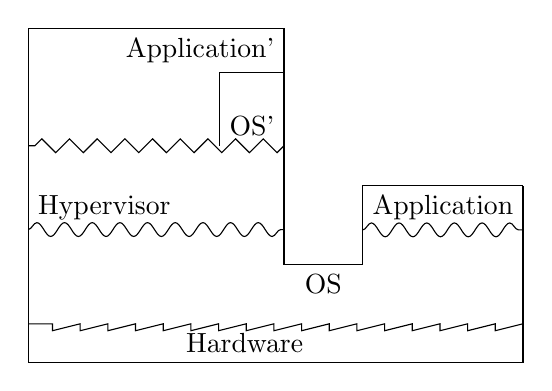
\begin{tikzpicture}
\path (-0.5,0) node[below left] (app-win) {Application'};
\path (-0.5,-1) node[below left] (win) {OS'};
\path (-0.5,-2) node[below left, text width=3cm] (mon) {Hypervisor};
\path (0.5,-2) node[below right] (app-lin) {Application};
\path (0,-3) node[below] (lin) {OS};
\path (-1,-4) node (hw) {Hardware};

\draw (0, -3) -|
	(node cs:name=mon, anchor=south east) -| (node cs:name=app-win,anchor=north east) -|
	(node cs:name=mon, anchor=south west);

\draw (node cs:name=win, anchor=south west) |- (node cs:name=app-win,anchor=south east);

\draw   (node cs:name=app-lin, anchor=north east) -- (node cs:name=app-lin, anchor=north west) |-
		(0, -3) ;

\draw   (node cs:name=hw, anchor=south) -| (node cs:name=mon, anchor=north west);
\draw   (node cs:name=hw, anchor=south) -| (node cs:name=app-lin, anchor=north east);

\draw [snake=zigzag] (node cs:name=win, anchor=south east) --
		(perpendicular cs:
		vertical line through  ={(mon.west)},
		horizontal line through={(win.south east)}
		);
\draw [snake=snake] (node cs:name=mon, anchor=south west) --
					(node cs:name=mon, anchor=south east) ;
\draw [snake=snake] (node cs:name=app-lin, anchor=south west) --
					(node cs:name=app-lin, anchor=south east) ;

\draw[snake=saw]
(perpendicular cs:
		vertical line through  ={(app-lin.east)},
		horizontal line through={(hw.north)}
		) --
(perpendicular cs:
		vertical line through  ={(mon.west)},
		horizontal line through={(hw.north)}
		);
\end{tikzpicture}

\end{document}
